\clearpage
\chapter{Shift Reduce Parser}

\section{Aim}
To design and construct a Shift Reduce Parser for a given language
\begin{algorithmic}[1]
	\State $E \quad \rightarrow \quad E \; + \; E$
	\State $E \quad \rightarrow \quad E \; - \; E$
	\State $E \quad \rightarrow \quad E \; * \; E$
	\State $E \quad \rightarrow \quad ( \; E \; )$
	\State $E \quad \rightarrow \quad i$
\end{algorithmic}




\section{Theory}
Shift-reduce parsing is a form of bottom-up parsing in which a stack holds
grammar symbols and an input buffer holds the rest of the string to be parsed.
The handle always appears at the top of the stack just before
it is identified as the handle.
A special symbol \$ to mark the bottom of the stack and also the right end of the
input. 

Initially, the stack is empty, and the string $w$ is on the input. During a left-to-right scan of the input string, the parser shifts zero or more
input symbols onto the stack, until it is ready to reduce a string of grammar
symbols on top of the stack. It then reduces to the head of the appropriate production. The parser repeats this cycle until it has detected an error or until
the stack contains the start symbol and the input is empty. Upon entering this configuration, the parser halts and announces successful
completion of parsing.

There are four possible actions a shift-reduce parser can make
\begin{enumerate}
	\item \textbf{Shift}.  Shift the next input symbol onto the top of the stack.
	\item \textbf{Reduce}. The right end of the string to be reduced must be at the top of
the stack. Locate the left end of the string within the stack and decide
with what nonterminal to replace the string.
	\item \textbf{Accept}. Announce successful completion of parsing.
	\item \textbf{Error}. Discover a syntax error and call an error recovery routine.
\end{enumerate}


\section{Algorithm}

\begin{algorithm}[!h]
	\caption{Computation of CLOSURE}
	\label{alg:closure}
	\begin{algorithmic}[1]
		\Procedure{CLOSURE}{I} \Comment{Returns set of Items}
			\State $J \gets I$
			\Repeat 
				\ForAll{item $A \rightarrow \alpha.B\beta$}
					\ForAll{production $B \rightarrow \gamma$ of $G$}
						\If{$B \rightarrow .\gamma$ is not in J}
							\State Add $B \rightarrow .\gamma$ to $J$
						\EndIf
					\EndFor
				\EndFor
			\Until{no more items are added to $J$ on one round}
			\State \Return $J$
		\EndProcedure
	\end{algorithmic}
\end{algorithm}

\begin{algorithm}[!h]
	\caption{Computation of the canonical collection of set of LR(0) items}
	\label{alg:LR0Items}
	\begin{algorithmic}[1]
		\Procedure{items}{G'}
			\State $C \gets \{ \Call{CLOSURE}{\{[S\ \rightarrow .S]\}}\}$ 
			\Repeat
			\ForAll{set of items $I \in C$}
				\ForAll{grammar symbol $X$}
					\If{$\Call{GOTO}{I,X}$ is not empty and not in $C$}
						\State Add \Call{GOTO}{I,X} to C
					\EndIf
				\EndFor
			\EndFor
			\Until{no new set of imtes are added to $C$ on a round}
		\EndProcedure
	\end{algorithmic}
\end{algorithm}

\begin{algorithm}[!h]
	\caption{LR-parsing}
	\label{alg:LRparser}
	\begin{algorithmic}[1]
		\State Let $a$ be the first symbol of $W\$$
		\While{1}
			\State Let $s$ be the state on top of the stack
			\If{$\Call{ACTION}{s,a} = shift \quad t$}
				\State push $t$ onto the stack
				\State let $a$ be the next input symbol
			\ElsIf{$\Call{ACTION}{s,a} = reduce \quad A \rightarrow \beta$}
				\State pop $|\beta|$ symbols off the stack
				\State let state $t$ now be on top of the stack
				\State push $\Call{GOTO}{t,A}$ onto the stack
				\State output the production $A \rightarrow \beta$
			\ElsIf{$\Call{ACTION}{s,a} = accept$}
				\State break \Comment{Parsing is done}
			\Else
				\State call error-recovery routine
			\EndIf
		\EndWhile
	\end{algorithmic}
\end{algorithm}

\break

\section{Grammar}
\subsection{Augmented Grammar}
\begin{algorithmic}[1]
	\setcounter{ALG@line}{-1}	
	\State $E' \quad \rightarrow \quad E$
	\State $E \quad \rightarrow \quad E \; + \; E$
	\State $E \quad \rightarrow \quad E \; - \; E$
	\State $E \quad \rightarrow \quad E \; * \; E$
	\State $E \quad \rightarrow \quad ( \; E \; )$
	\State $E \quad \rightarrow \quad i$
\end{algorithmic}

\break
\subsection{LR(0) Automaton}
\begin{figure}[!h]
	\centering
	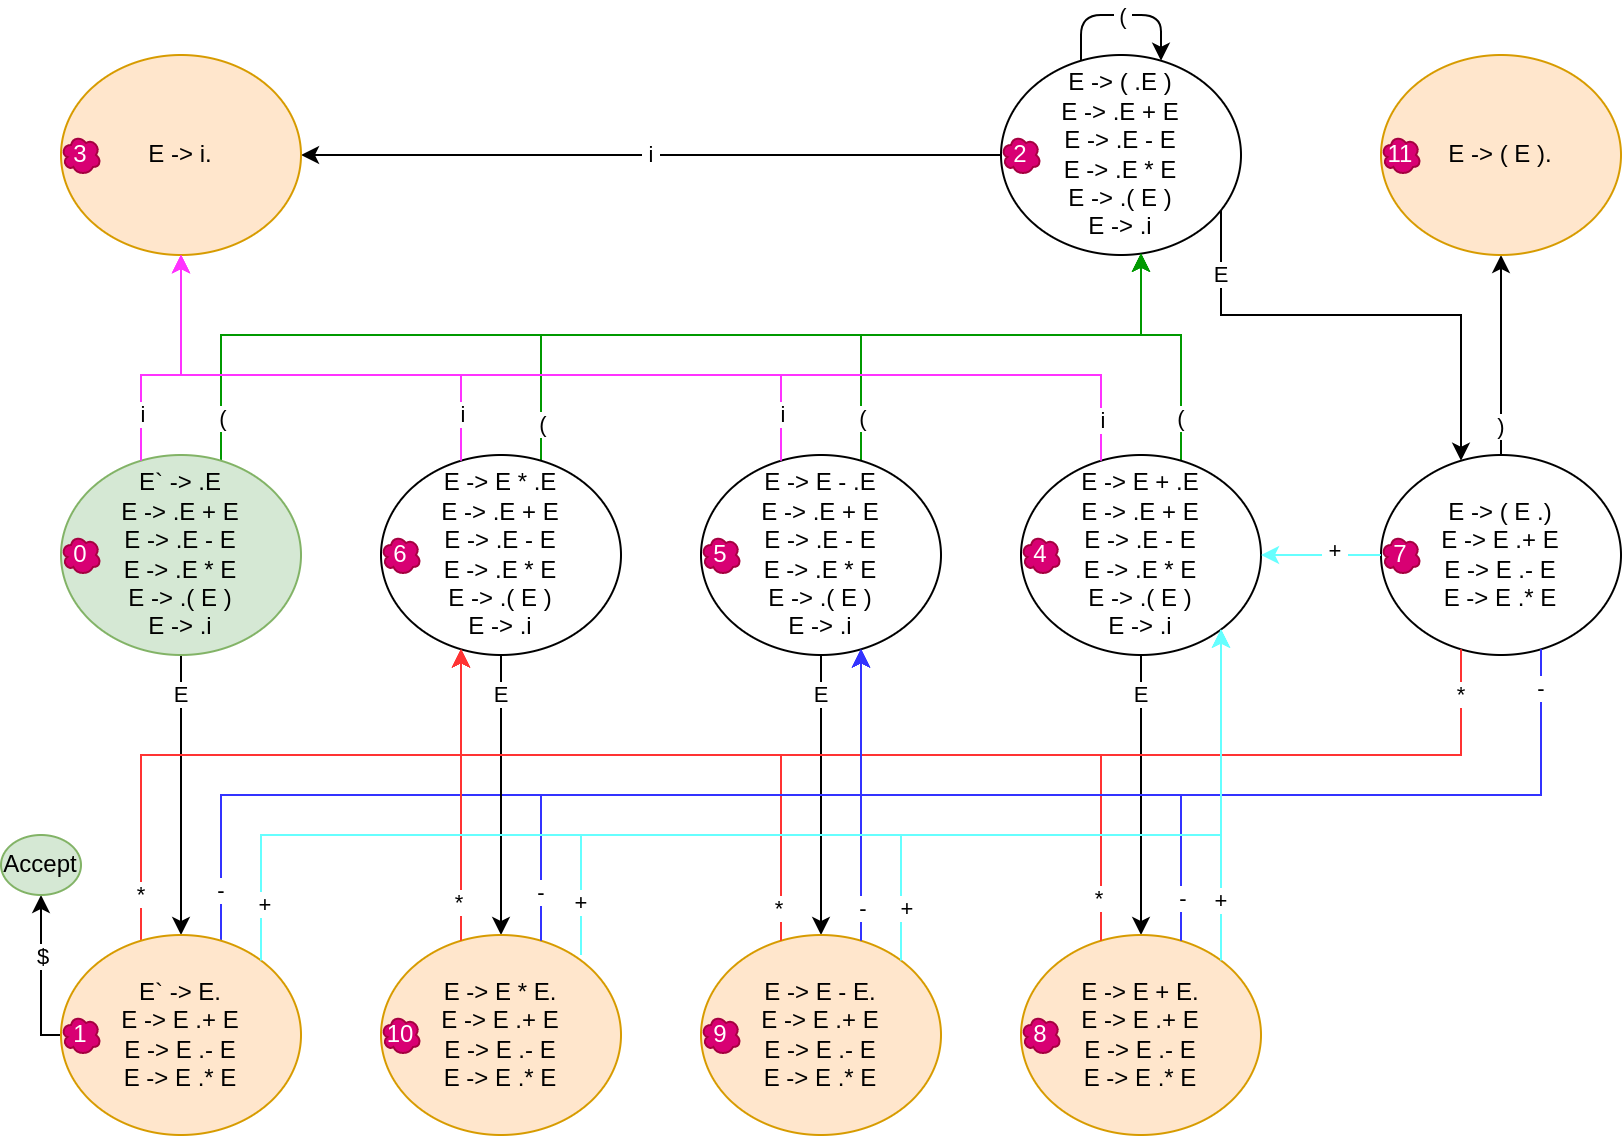
\includegraphics[width=\textwidth]{../EXP7/automaton.png}
	\caption{LR(0) Automaton}
\end{figure}

\subsection{First \& Follow}
\begin{table}[!h]
	\centering
	\begin{tabular}{|lll|}
		\hline
		\multicolumn{3}{|c|}{\textbf{FIRST / FOLLOW table}}                      \\ \hline
		\multicolumn{1}{|c|}{\textbf{Nonterminal}} & \multicolumn{1}{c|}{\textbf{FIRST}} & \multicolumn{1}{c|}{\textbf{FOLLOW}} \\ \hline
		\multicolumn{1}{|l|}{E'} & \multicolumn{1}{l|}{\{(,i\}} & \{\$\}         \\ \hline
		\multicolumn{1}{|l|}{E}  & \multicolumn{1}{l|}{\{(,i\}} & \{\$,+,-,*,)\} \\ \hline
	\end{tabular}
\end{table}

\break
\subsection{Parse-Table}
\begin{table}[!h]
	\centering
	\resizebox{\textwidth}{!}{%
		\begin{tabular}{|cccccccccc|}
			\hline
			\multicolumn{10}{|c|}{\textbf{LR table}} \\ \hline
			\multicolumn{1}{|c|}{} &
			\multicolumn{7}{c|}{\textbf{ACTION}} &
			\multicolumn{2}{c|}{\textbf{GOTO}} \\ \cline{2-10} 
			\multicolumn{1}{|c|}{\multirow{-2}{*}{\textbf{State}}} &
			\multicolumn{1}{c|}{\textbf{+}} &
			\multicolumn{1}{c|}{\textbf{-}} &
			\multicolumn{1}{c|}{\textbf{*}} &
			\multicolumn{1}{c|}{\textbf{(}} &
			\multicolumn{1}{c|}{\textbf{)}} &
			\multicolumn{1}{c|}{\textbf{i}} &
			\multicolumn{1}{c|}{\textbf{\$}} &
			\multicolumn{1}{c|}{\textbf{E1}} &
			\multicolumn{1}{c|}{\textbf{E}} \\ \hline
			\multicolumn{1}{|c|}{0} &
			\multicolumn{1}{c|}{} &
			\multicolumn{1}{c|}{} &
			\multicolumn{1}{c|}{} &
			\multicolumn{1}{c|}{s2} &
			\multicolumn{1}{c|}{} &
			\multicolumn{1}{c|}{s3} &
			\multicolumn{1}{c|}{} &
			\multicolumn{1}{c|}{} &
			1 \\ \hline
			\multicolumn{1}{|c|}{1} &
			\multicolumn{1}{c|}{s4} &
			\multicolumn{1}{c|}{s5} &
			\multicolumn{1}{c|}{s6} &
			\multicolumn{1}{c|}{} &
			\multicolumn{1}{c|}{} &
			\multicolumn{1}{c|}{} &
			\multicolumn{1}{c|}{acc} &
			\multicolumn{1}{c|}{} &
			\\ \hline
			\multicolumn{1}{|c|}{2} &
			\multicolumn{1}{c|}{} &
			\multicolumn{1}{c|}{} &
			\multicolumn{1}{c|}{} &
			\multicolumn{1}{c|}{s2} &
			\multicolumn{1}{c|}{} &
			\multicolumn{1}{c|}{s3} &
			\multicolumn{1}{c|}{} &
			\multicolumn{1}{c|}{} &
			7 \\ \hline
			\multicolumn{1}{|c|}{3} &
			\multicolumn{1}{c|}{r5} &
			\multicolumn{1}{c|}{r5} &
			\multicolumn{1}{c|}{r5} &
			\multicolumn{1}{c|}{} &
			\multicolumn{1}{c|}{r5} &
			\multicolumn{1}{c|}{} &
			\multicolumn{1}{c|}{r5} &
			\multicolumn{1}{c|}{} &
			\\ \hline
			\multicolumn{1}{|c|}{4} &
			\multicolumn{1}{c|}{} &
			\multicolumn{1}{c|}{} &
			\multicolumn{1}{c|}{} &
			\multicolumn{1}{c|}{s2} &
			\multicolumn{1}{c|}{} &
			\multicolumn{1}{c|}{s3} &
			\multicolumn{1}{c|}{} &
			\multicolumn{1}{c|}{} &
			8 \\ \hline
			\multicolumn{1}{|c|}{5} &
			\multicolumn{1}{c|}{} &
			\multicolumn{1}{c|}{} &
			\multicolumn{1}{c|}{} &
			\multicolumn{1}{c|}{s2} &
			\multicolumn{1}{c|}{} &
			\multicolumn{1}{c|}{s3} &
			\multicolumn{1}{c|}{} &
			\multicolumn{1}{c|}{} &
			9 \\ \hline
			\multicolumn{1}{|c|}{6} &
			\multicolumn{1}{c|}{} &
			\multicolumn{1}{c|}{} &
			\multicolumn{1}{c|}{} &
			\multicolumn{1}{c|}{s2} &
			\multicolumn{1}{c|}{} &
			\multicolumn{1}{c|}{s3} &
			\multicolumn{1}{c|}{} &
			\multicolumn{1}{c|}{} &
			10 \\ \hline
			\multicolumn{1}{|c|}{7} &
			\multicolumn{1}{c|}{s4} &
			\multicolumn{1}{c|}{s5} &
			\multicolumn{1}{c|}{s6} &
			\multicolumn{1}{c|}{} &
			\multicolumn{1}{c|}{s11} &
			\multicolumn{1}{c|}{} &
			\multicolumn{1}{c|}{} &
			\multicolumn{1}{c|}{} &
			\\ \hline
			\multicolumn{1}{|c|}{8} &
			\multicolumn{1}{c|}{\cellcolor[HTML]{FFC0CB}s4 / \sout{r1}} &
			\multicolumn{1}{c|}{\cellcolor[HTML]{FFC0CB}s5 / \sout{r1}} &
			\multicolumn{1}{c|}{\cellcolor[HTML]{FFC0CB}s6 / \sout{r1}} &
			\multicolumn{1}{c|}{} &
			\multicolumn{1}{c|}{r1} &
			\multicolumn{1}{c|}{} &
			\multicolumn{1}{c|}{r1} &
			\multicolumn{1}{c|}{} &
			\\ \hline
			\multicolumn{1}{|c|}{9} &
			\multicolumn{1}{c|}{\cellcolor[HTML]{FFC0CB}s4 / \sout{r2}} &
			\multicolumn{1}{c|}{\cellcolor[HTML]{FFC0CB}s5 / \sout{r2}} &
			\multicolumn{1}{c|}{\cellcolor[HTML]{FFC0CB}s6 / \sout{r2}} &
			\multicolumn{1}{c|}{} &
			\multicolumn{1}{c|}{r2} &
			\multicolumn{1}{c|}{} &
			\multicolumn{1}{c|}{r2} &
			\multicolumn{1}{c|}{} &
			\\ \hline
			\multicolumn{1}{|c|}{10} &
			\multicolumn{1}{c|}{\cellcolor[HTML]{FFC0CB}s4 / \sout{r3}} &
			\multicolumn{1}{c|}{\cellcolor[HTML]{FFC0CB}s5 / \sout{r3}} &
			\multicolumn{1}{c|}{\cellcolor[HTML]{FFC0CB}s6 / \sout{r3}} &
			\multicolumn{1}{c|}{} &
			\multicolumn{1}{c|}{r3} &
			\multicolumn{1}{c|}{} &
			\multicolumn{1}{c|}{r3} &
			\multicolumn{1}{c|}{} &
			\\ \hline
			\multicolumn{1}{|c|}{11} &
			\multicolumn{1}{c|}{r4} &
			\multicolumn{1}{c|}{r4} &
			\multicolumn{1}{c|}{r4} &
			\multicolumn{1}{c|}{} &
			\multicolumn{1}{c|}{r4} &
			\multicolumn{1}{c|}{} &
			\multicolumn{1}{c|}{r4} &
			\multicolumn{1}{c|}{} &
			\\ \hline
		\end{tabular}%
	}
\end{table}


\subsection{Parse-Tree}
\begin{figure}[!h]
	\centering
	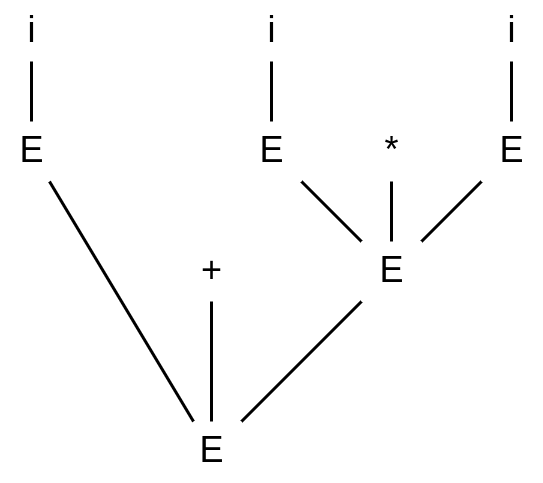
\includegraphics[height=2in]{../EXP7/parse_tree.png}
	\caption{Bottom up parser for i+i*i}
\end{figure}

\break
\section{C-Program}
\lstinputlisting[style=CStyle,language=C]{../EXP7/shiftreducer.c}

\section{Output}
Output1
\lstinputlisting[style=plain]{../EXP7/output1.txt}
Output2
\lstinputlisting[style=plain]{../EXP7/output2.txt}

\section{Result}
The program compiled and successfully parsed a string via Simple LR parser for the given grammar.